%=============================--A--=============================%
%\definecolor{green}{rgb}{0.1,0.1,0.1}
\subsection{E.2 Análise do sistema BPSK}
\label{sec:analiseBPSK}
\vskip -0.5em
\begin{table}[H]
\caption{Taxa de erro de \textit{bit} em função da \textit{Loop Bandwidth}, para cada \textit{noise voltage}.}
\vskip -0.5em
\label{tab:bpsk}
\hspace*{-0.75cm}\begin{tabular}{|c|c|c|c|c|c|c|c|c|c|}
\hline
Loop BW/Noise & 0.0 & 0.5 & 1.0 & 1.5 & 2.0 & 2.5 & 3.0 & 3.5 & 4.0 \\
\hline\hline
0.006 &\cellcolor{green!25}0.0\% & 1.4\% & 9.7\% & 19.0\% & 25.5\% & 30.6\% & 34.7\% & 38.0\% & 39.4\% \\
\hline
0.012 &\cellcolor{green!25}0.0\% & 1.4\% & 9.7\% & 19.0\% & 25.0\% & 29.6\% & 34.3\% & 35.6\% & 38.0\% \\
\hline
0.018 &\cellcolor{green!25}0.0\% & 1.4\% & 9.7\% & 19.4\% & 25.0\% & 28.7\% & 33.3\% & 36.6\% & \cellcolor{green!25}33.8\% \\
\hline
0.024 &\cellcolor{green!25}0.0\% & 1.4\% & 9.7\% & 19.4\% & \cellcolor{green!25}24.5\% & 29.6\% & 34.7\% & 39.4\% & 34.3\% \\
\hline
0.03 &\cellcolor{green!25}0.0\% & 1.4\% & 9.7\% & 19.0\% & \cellcolor{green!25}24.5\% & 29.6\% & 34.7\% & 34.3\% & 37.5\% \\
\hline
0.036 &\cellcolor{green!25}0.0\% & 1.4\% & 9.7\% & 19.0\% & 25.0\% & 28.7\% & \cellcolor{green!25}31.0\% & \cellcolor{green!25}33.3\% & 38.9\% \\
\hline
0.042 &\cellcolor{green!25}0.0\% & 1.4\% & 9.7\% & 18.5\% & 25.0\% & 37.0\% & 32.4\% & 34.3\% & 39.8\% \\
\hline
0.048 &\cellcolor{green!25}0.0\% & 1.4\% & 9.3\% & 18.5\% & \cellcolor{green!25}24.5\% & \cellcolor{green!25}28.2\% & \cellcolor{green!25}31.0\% & 36.1\% & 44.9\% \\
\hline
0.054 &\cellcolor{green!25}0.0\% &\cellcolor{green!25}0.9\% & 9.7\% & 18.5\% & 35.2\% & 31.5\% & \cellcolor{green!25}31.0\% & 38.0\% & 39.4\% \\
\hline
0.06 &\cellcolor{green!25}0.0\% &\cellcolor{green!25}0.9\% & 9.3\% & 20.8\% & 25.0\% & 28.7\% & 34.7\% & 50.0\% & 43.1\% \\
\hline
0.066 &\cellcolor{green!25}0.0\% &\cellcolor{green!25}0.9\% & 9.3\% & 20.4\% & 25.0\% & \cellcolor{green!25}28.2\% & 34.7\% & 40.3\% & 41.2\% \\
\hline
0.072 &\cellcolor{green!25}0.0\% &\cellcolor{green!25}0.9\% & 8.8\% & 19.9\% & 25.9\% & 27.3\% & 33.3\% & 56.0\% & 55.1\% \\
\hline
0.078 &\cellcolor{green!25}0.0\% &\cellcolor{green!25}0.9\% & 10.6\% & 19.0\% & 27.3\% & 29.2\% & 40.7\% & 40.3\% & 44.4\% \\
\hline
0.084 &\cellcolor{green!25}0.0\% &\cellcolor{green!25}0.9\% & 12.0\% & 19.4\% & 26.9\% & 29.6\% & 37.5\% & 35.6\% & 42.6\% \\
\hline
0.09 &\cellcolor{green!25}0.0\% &\cellcolor{green!25}0.9\% & 11.6\% & \cellcolor{green!25}16.7\% & 27.8\% & 38.4\% & 41.2\% & 56.9\% & 51.4\% \\
\hline
0.096 &\cellcolor{green!25}0.0\% &\cellcolor{green!25}0.9\% & 11.6\% & 17.1\% & 25.9\% & 38.4\% & 48.1\% & 32.4\% & 49.5\% \\
\hline
0.102 &\cellcolor{green!25}0.0\% &\cellcolor{green!25}0.9\% & 10.2\% & 19.9\% & 25.5\% & 41.7\% & 44.4\% & 42.1\% & 50.5\% \\
\hline
0.108 &\cellcolor{green!25}0.0\% &\cellcolor{green!25}0.9\% & 9.7\% & 20.4\% & 25.5\% & 38.4\% & 49.1\% & 46.3\% & 54.2\% \\
\hline
0.114 &\cellcolor{green!25}0.0\% &\cellcolor{green!25}0.9\% & 8.8\% & 23.1\% & 30.1\% & 37.0\% & 47.7\% & 42.1\% & 50.0\% \\
\hline
0.12 &\cellcolor{green!25}0.0\% &\cellcolor{green!25}0.9\% & \cellcolor{green!25}7.4\% & 18.5\% & 39.8\% & 44.4\% & 51.9\% & 48.1\% & 49.5\% \\
\hline
0.126 &\cellcolor{green!25}0.0\% &\cellcolor{green!25}0.9\% & 7.9\% & 21.3\% & 40.7\% & 33.3\% & 48.6\% & 47.7\% & 46.3\% \\
\hline
0.132 &\cellcolor{green!25}0.0\% &\cellcolor{green!25}0.9\% & 9.3\% & 19.9\% & 44.0\% & 33.3\% & 47.2\% & 53.7\% & 48.6\% \\
\hline
0.138 &\cellcolor{green!25}0.0\% &\cellcolor{green!25}0.9\% & 10.6\% & 21.8\% & 37.5\% & 37.0\% & 48.1\% & 47.7\% & 50.0\% \\
\hline
0.144 &\cellcolor{green!25}0.0\% &\cellcolor{green!25}0.9\% & 8.3\% & \cellcolor{green!25}16.7\% & 37.5\% & 44.9\% & 50.5\% & 44.0\% & 53.7\% \\
\hline
0.15 &\cellcolor{green!25}0.0\% &\cellcolor{green!25}0.9\% & 8.3\% & 19.0\% & 38.0\% & 39.4\% & 43.1\% & 44.9\% & 53.2\% \\
\hline
0.156 &\cellcolor{green!25}0.0\% &\cellcolor{green!25}0.9\% & 10.6\% & 17.1\% & 28.2\% & 36.1\% & 47.7\% & 53.2\% & 50.5\% \\
\hline
0.162 &\cellcolor{green!25}0.0\% &\cellcolor{green!25}0.9\% & 9.7\% & 19.0\% & 44.0\% & 35.2\% & 44.4\% & 44.4\% & 53.7\% \\
\hline
0.168 &\cellcolor{green!25}0.0\% &\cellcolor{green!25}0.9\% & 9.7\% & 21.8\% & 31.9\% & 48.1\% & 41.7\% & 52.3\% & 51.9\% \\
\hline
0.174 &\cellcolor{green!25}0.0\% &\cellcolor{green!25}0.9\% & 9.3\% & 27.8\% & 39.8\% & 43.1\% & 53.7\% & 50.5\% & 44.4\% \\
\hline
0.18 &\cellcolor{green!25}0.0\% &\cellcolor{green!25}0.9\% & 8.8\% & 31.0\% & 48.6\% & 50.5\% & 45.4\% & 53.2\% & 47.2\% \\
\hline
0.186 &\cellcolor{green!25}0.0\% &\cellcolor{green!25}0.9\% & 9.3\% & 30.6\% & 42.1\% & 44.4\% & 52.3\% & 57.9\% & 46.8\% \\
\hline
0.192 &\cellcolor{green!25}0.0\% &\cellcolor{green!25}0.9\% & 11.6\% & 21.8\% & 48.1\% & 42.6\% & 51.9\% & 52.3\% & 49.5\% \\
\hline
0.198 &\cellcolor{green!25}0.0\% & 1.4\% & \cellcolor{green!25}7.4\% & 21.3\% & 45.8\% & 52.8\% & 45.4\% & 46.8\% & 47.2\% \\
\hline
0.204 &\cellcolor{green!25}0.0\% & 1.4\% & 8.3\% & 39.8\% & 44.4\% & 57.9\% & 51.4\% & 49.1\% & 51.9\% \\
\hline
0.21 &\cellcolor{green!25}0.0\% &\cellcolor{green!25}0.9\% & 16.2\% & 42.6\% & 34.3\% & 30.6\% & 50.5\% & 45.8\% & 50.5\% \\
\hline
0.216 &\cellcolor{green!25}0.0\% & 1.9\% & 23.6\% & 40.7\% & 43.5\% & 40.3\% & 43.5\% & 45.8\% & 50.5\% \\
\hline
0.222 &\cellcolor{green!25}0.0\% & 1.4\% & 13.9\% & 53.2\% & 44.0\% & 53.2\% & 51.9\% & 44.4\% & 50.9\% \\
\hline
0.228 &\cellcolor{green!25}0.0\% & 1.9\% & 12.5\% & 19.9\% & 36.6\% & 48.6\% & 47.2\% & 48.1\% & 49.5\% \\
\hline
0.234 &\cellcolor{green!25}0.0\% & 8.3\% & 10.6\% & 31.9\% & 25.9\% & 47.2\% & 48.6\% & 45.8\% & 54.6\% \\
\hline
0.24 &\cellcolor{green!25}0.0\% &\cellcolor{green!25}0.9\% & 11.1\% & 38.9\% & 36.6\% & 44.9\% & 44.4\% & 50.5\% & 51.9\% \\
\hline
0.246 &\cellcolor{green!25}0.0\% & 1.4\% & 12.5\% & 38.4\% & 46.8\% & 49.1\% & 52.8\% & 50.5\% & 42.1\% \\
\hline
0.252 &\cellcolor{green!25}0.0\% & 1.4\% & 28.7\% & 21.8\% & 49.5\% & 44.9\% & 45.4\% & 43.5\% & 52.3\%\\
\hline
\end{tabular}
\end{table}

%---
\begin{figure}[H]
    \centering
    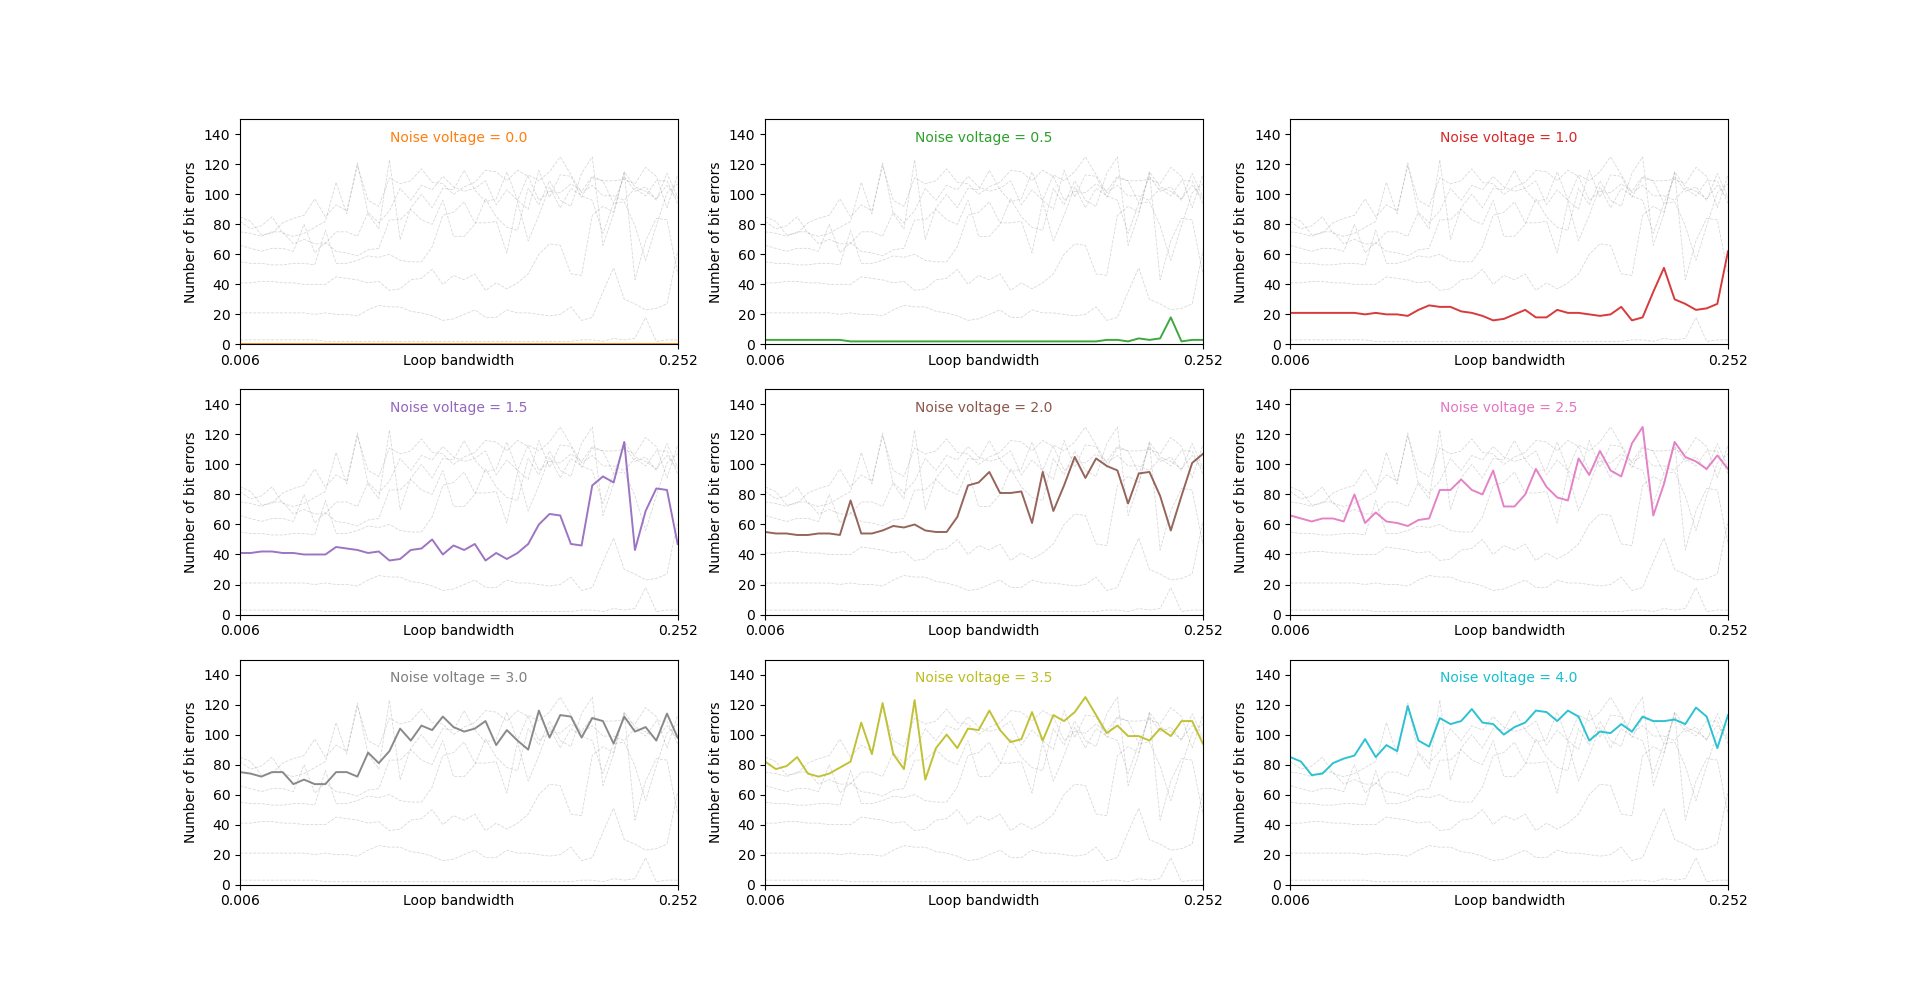
\includegraphics[width=1\linewidth]{img/analise/BPSK_9.png}
    \caption{Evolução do número de erros de \textit{bit} para cada \textit{noise voltage}, em função da \textit{Loop Bandwidth}.}
    \label{fig:bpsk9}
\end{figure}

\noindent\fcolorbox{black}{white}{%
        \minipage[t]{\dimexpr\linewidth-2\fboxsep-2\fboxrule\relax}
            \textbf{Observação 1} $\rightarrow$ Verifica-se, como esperado, um número de erros cada vez mais prevalente e mais oscilante para valores de \textit{Loop Bandwidth} cada vez mais distantes de zero (distanciamento da gama ótima de valores\cite{symbolsync-gnuradio} discutida anteriormente na \hyperref[subsubsec:symbol-sync]{secção 3.1}). É também de salientar a proporcionalidade observada (e expectável) do número de erros de \textit{bit} com o patamar de ruído (aumento da dificuldade em detetar o pulso no seio do ruído $\implies$ maior taxa de erro de \textit{bit}).
        \endminipage}

\vskip 1em
\noindent\fcolorbox{black}{white}{%
        \minipage[t]{\dimexpr\linewidth-2\fboxsep-2\fboxrule\relax}
            \textbf{Observação 2} $\rightarrow$ Para cada gráfico é aparente uma zona de maior estabilidade (número de erros bastante próximos) que tende a contrair e a mutar para uma extensão cada vez mais instável, com o aumento da \textit{noise voltage}. 
        \endminipage}

\vskip 1em
\noindent\fcolorbox{black}{white}{%
        \minipage[t]{\dimexpr\linewidth-2\fboxsep-2\fboxrule\relax}
            \textbf{Nota} $\rightarrow$ Encontram-se a \textcolor{green}{verde} na tabela os valores da \textit{Loop Bandwidth} que minimizam a taxa de erro de \textit{bit} para cada patamar de ruído no sistema BPSK projetado. A segunda observação é corroborada por estes valores \textit{highlighted}, dado que o valor ótimo de \textit{Loop Bandwidth} aparenta tender para valores nominalmente mais próximos de zero com o aumento da \textit{noise voltage}. 
        \endminipage}